
\section{Problem Statement}
We now present the formal problem statement along with our assumptions.

\subsection{Problem Setup}
\sys takes as input a dirty training dataset $(X_{train}, Y_{train})$ where both the features $X_{train}$ and labels $Y_{train}$ may have errors, as well as a test dataset $(X_{test}, Y_{test})$ where the features may contain errors however the labels $Y_{test}$ are correct.  Although the training labels may contain errors, the test labels must be clean to ensure an unbiased measure of accuracy that is not affected by data cleaning operations.  Such labels may be collected as part of a gold standard dataset~\cite{marcus2015crowdsourced} or by cross-referencing the data with other sources~\cite{li2012truth}.  
Labels often represent directly observed phenomena such as (e.g., purchased/not purchased), while features are integrated from multiple disparate sources and subject to frequent change.
Let a record $r_i = (x_i,y_i) \in (X_{train},Y_{train})$ denote the features along with its corresponding (possibly null) label, and $r_i.y$ denote the label for the record.    Furthermore, the features may be categorical, or string-valued, in addition to numerical.

\begin{example}[Notation]
In Example~\ref{ex:lead}, the attributes $name$, $n\_emp$, $industry$, and $region$ define the schema of $X_{train,test}$, and the attribute $successful$ corresponds to the labels $Y_{train,test}$.
\end{example}

Let a classifier $C(r_i) = r_i'$ be a function that takes as input a record $r_i$ and sets $r_i.y$ to the predicted label value.
A classifier predicts $(x_i, y_i) \in (X_{test}, Y_{test})$ correctly if  $C((x_i, null)).y = y_i$.  $C$'s test accuracy is defined as the fraction of correctly predicted test records:
\[
acc(C) = \frac{|\{\forall x,y \in (X_{test}, X_{test})~:~ C((x, null)).y = y\}|}{|Y_{test}|}
\]
To generate a classifier, the user provides \textsf{train}($X_{train}, Y_{train}$) that return a classifier $C$. We model \textsf{train}($\cdot$) as a black-box and assume that the function internally performs any necessary featurization.

\begin{example}[Classification]\sloppy
The classifier $C$ can be a support vector machine predicting whether $successful = true$ based on a feature vector derived from
$name$, $n\_emp$, $industry$, and $region$.
\end{example}

\subsection{Detection and Repair Libraries}\label{s:detectorgen}
We assume that the user provides a library of detector generators $\mathcal{D} = \{d_1,\cdots\}$ and a repair library $\mathcal{F} = \{f_1,\cdots\}$.  \sys uses $\mathcal{D}$ to generate predicates that identify candidate dirty records, and selects the appropriate repair functions in $\mathcal{F}$ to those records.  

\subsubsection{Detection Generators and Predicates}
We define a predicate $p_i$ as a Boolean expression over an input record that returns the set of referenced attributes if it evaluates to $true$ and an empty set otherwise.  Based on this definition, we say that $r$ is a candidate dirty record if $p_i(r) \ne \emptyset$. For instance, $p_i(r) = r.n\_emp \le 0$ is an example of the former: if a company record contains $0$ employees, then the predicate will return $\{n\_emp\}$.  From an API perspective, we need a more expressive model than pre-defined Boolean expressions: 

First, predicate expressions may reference combinations of attributes.  For instance, if we knew that there are no oil and natural gas companies in the northwest, the predicate $p_i(r) =  (r.region == USNW \wedge r.industry \in ('OIL','NG'))$ would return $\{region, industry\}$ if such a company were detected.
Second, predicates may apply transformation functions over the input data.  For instance, the following predicate first featurizes the record using a function $g$, and applies a threshold to the first element of the feature vector: $p_i(r) = g(r)[0] > 10$.  
Third, predicate expressions may contain aggregate expressions that are computed over all records in the training dataset $X_{train}$.  For instance, the following predicate performs Quantitative Error Detection~\cite{hellerstein2008quantitative} by checking whether the record's $n\_emp$ value is further than $5$ standard deviations of the mean: 
$$p_i(r) = |r.n\_emp - avg(r.n\_emp)| > 5\times stddev(r.n\_emp)$$

To address these problems we define a detector generator $d_i$ is a function that takes the full training set as input and returns a predicate $p_i$. 
In thise sense, predicates can be derived or learned from previous data.

\subsubsection{Repair Functions}
Each repair function $f_i \in \mathcal{F}$ is a function that takes a record as input and modifies the record's attributes.  We consider two types of repairs:  {\it data repairs} are applied to the training data prior to running the training procedure, while {\it prediction repairs} modify the label of the records {\it after} the classifier makes a prediction.   

{\it Data repairs} modify the values of a training record in response to a detected error (due to a predicate).  These repair functions are free to modify the record's features, label, or simply delete the record from the training dataset.  

{\it Prediction repairs}, on the other hand, take as input the non-transformed record along with the classifier prediction, and replaces the prediction with a default value.  This is useful when the input record is too corrupted to provide a reliable prediction.  For instance, the NFL play-by-play dataset describe in Section~\ref{s:exp}, some input records contain almost all null attributes and it is more accurate to default the prediction to the most frequent label rather than attempting a repair.

Note that this section formalizes an API for these operations and subsequent sections provide one instantiation of this library.

\subsubsection{Conditional Repairs}
\sys applies repair functions to specific sets of records through the use of {\it conditional repairs}.  A conditional repair $l_k = (p_k, f_k)$ is a tuple where $p_k = d_i(X_{train}, Y_{train})$ is the output of a detector generator and $f_k \in \mathcal{F}$ is a repair function. 
A conditional repair is compiled into generation procedure that returns a repair function; the repair function takes as input a possibly cleaned record $r$, along with its original uncleaned version $r_{orig}$:
{\small\begin{verbatim}
    def generate_repair(p, f):
      def repair(r, r_orig):
        if p(r): r = f(r)   
        return r 
      return apply
\end{verbatim}}

\begin{example}[Value Canonicalization]\sloppy
The following script canonicalizes different representations for Western United States:
{\small\begin{verbatim}
    def repair(r, r_orig):
      if r.region in ('USWest', 'USWESTERN'):
        r.region = 'USW'
      return r
\end{verbatim}}
\end{example}

\vspace{0.25em}
\begin{example}[Default Prediction]\sloppy
The following script represents a conditional prediction repair that predicts $false$ if the company name is missing.  Note that the predicate is applied on the original non-cleaned record. However the classifier takes as input the cleaned version.
{\small\begin{verbatim}
    def repair(r, r_orig):
      if r_orig.name == None:
        r.y = False
        return r
      return C(r)
\end{verbatim}}
\end{example}

\noindent Finally, let $L = (l_1,\cdots,l_n)$ be a sequence of conditional data and prediction repairs that \sys generates. 
$L$ is an element in a finite universe of possible repairs denoted by $\mathcal{L}=\mathcal{D}\times\mathcal{F}$.
To apply the repairs, \sys first partitions the $L$ into two subsequences $L^d = (l_i \in L | l_i$ is data repair$)$ and $L^p = (l_i \in L | l_i$ is prediction repair$)$.  During the training phase, we apply the data repairs in sequence over the training dataset prior to training the classifier:
\begin{align}
(X'_{train}, Y'_{train}) = \{L^d(r, r) | r \in (X_{train}, Y_{train}) \}\\
C = train((X'_{train}, Y'_{train})\\
L^d(r, r) = l_k(l_{k-1}(\cdots l_1(r, r), r) r) | l_i \in L^d
\end{align}

Finally, \sys constructs the final classifier $C_{L}$ by combining the prediction repairs $L^p$ with the trained classifier $C$.  It first identifies the last prediction repair $l^* \in L^p$ whose predicate matches the test record.  
$$l^* = \argmax_{l_i \in L^p \wedge l_i(r) = true} i$$
If no such prediction repair is found, \sys  returns the classifier prediction on the cleaned record, otherwise it applies $l^*$:
$$C_{L}(r) = \begin{cases}
    C(L^d(r, r))& \text{if } l^*\textrm{\ not\ found}\\
    l^*(L^d(r, r), r) & \text{otherwise}
\end{cases}$$

\subsection{Scope and Assumptions}
As a class of errors, we focus on domain integrity constraints, i.e., a set of allowed values in each attribute's domain--an error being defined as an attribute value not in this set.
Given a violation, we assume that each of the repair actions sets the attribute to an allowed value.
This assumption avoids a fixed-point iteration, also called the ``chase algorithm''~\cite{aho1979theory}, which repairs that cause additional errors.
This greatly simplifies the specification of $\mathcal{L}$ the set of possible data cleaning operations--in our experiments, $|\mathcal{L}|$ varied from $192$ to $1076$.
Next, we assume that each record in a relation corresponds to a single example (features and labels), and the analyst wants to learn a classifier that predicts labels from features.
Finally, we assume that the labels of the test data are clean since \sys relies on uncorrupted labels to estimate the model's accuracy.

\subsection{Problem Statement}
Given these assumptions, we define the repair selection problem:

\begin{problem}[\sys Repair Selection]\sloppy
Given $(X_{train}, Y_{train})$, $(X_{test}, Y_{test})$, a library of detector generators $\mathcal{D}$ and of repair functions $\mathcal{F}$, and a training procedure $train$, identify the optimal sequence $L^*$ of $B$ conditional repairs such that the resulting classifier $C_{L^*}$  maximizes prediction accuracy on $(X_{test}, Y_{test})$:
$$L^* = \argmax_{L \in \mathcal{D}\times\mathcal{F}} acc(C_L)$$
\end{problem}

Greedy solutions that select the top $B$ individual condition repairs will often fail since they might select highly correlated repairs (e.g., imputing a missing value with the mean, and the median).
Instead, it is desirable for an approach to take the mispredictions from previous conditional repairs into account.  This is the reason we applied a boosting-based approach towards selecting conditional repairs, described in the next section~\cite{schapire2003boosting}.

\begin{figure}\centering
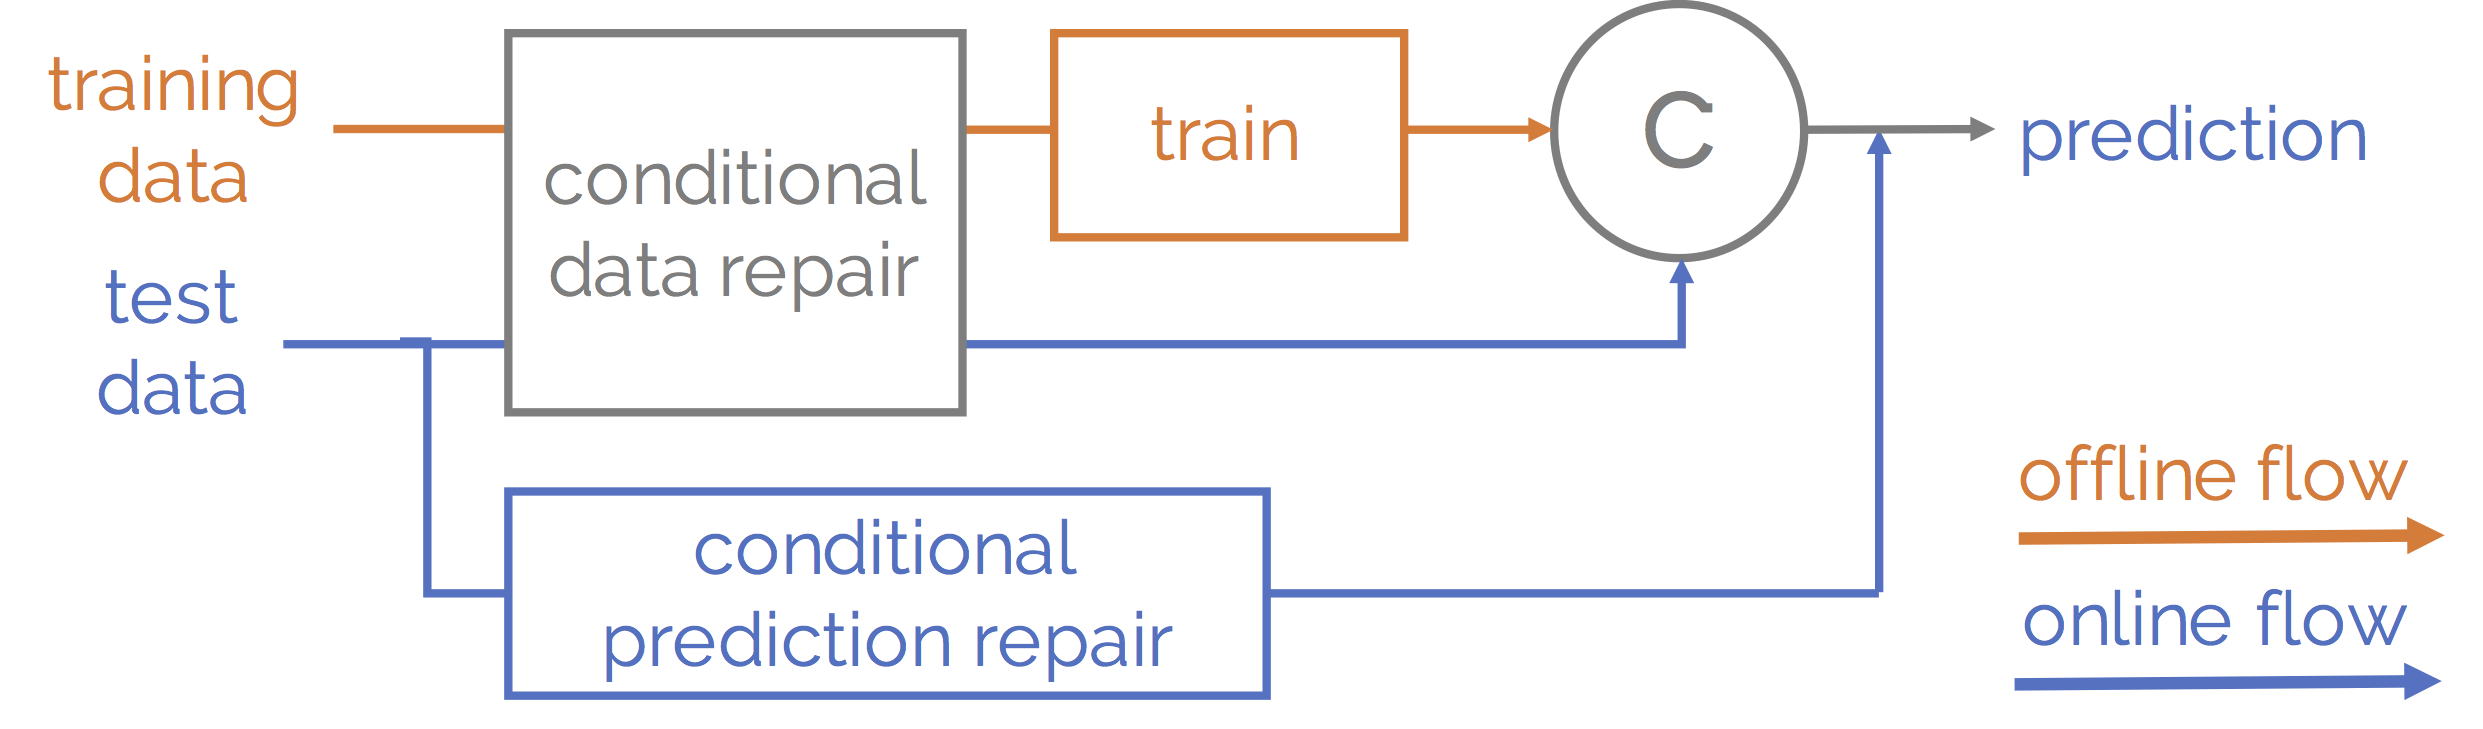
\includegraphics[width=\columnwidth]{figures/workflow.png}
\caption{Offline (\orange{orange}) and online (\blue{blue}) workflows.}
\label{fig:workflow}
\end{figure}

Figure~\ref{fig:workflow} summarizes the training and prediction workflows given the optimal sequence of conditional repairs $\mathcal{L}^*$.  The \orange{orange line} depicts the training process, which first applies the conditional data repairs to the training dataset, and calls \texttt{train()} to generate classifier $C$.  The \blue{blue lines} depict how \sys generates a prediction for a test record: the classifier $C$ makes a prediction using the record cleaned by the conditional data repairs.  In addition, the conditional prediction repair checks the uncleaned test record to decide whether to return the classifier prediction or a default value.


\iffalse
\vspace{0.25em}
\noindent \textbf{Composition Rules: } \sys studies composing data cleaning operations to maximize predictive model accuracy trained on the cleaned data. Now, we need to formalize what it means to compose two data cleaning operations $l_1$ and $l_2$. Recall, that each data cleaning operation is a two-tuple of a predicate and cleaning action $(p, a)$. We define the composition of two operations $l_1=(p_1, a_1)$ and $l_2=(p_2, a_2)$ as generating two new operations (intersection of the predicates, and applying each respective action):
\ewu{is this correct?  should it be $p_1 \wedge p_2$, $p_i \wedge not p_2$
\[
l_1 \circ l_2 := \{(p_1 \wedge p_2, a_1), (p_1 \wedge p_2, a_2)\}
\]
Based on this definition, we can define a restricted library $\mathcal{L}_{\mid l_i}$ that is generated by $l_i$ composed with each of the members of the library:
\[\mathcal{L}_{\mid l_i} = \bigcup_{\forall j \ne i \in \mathcal{L}} l_i \circ l_j \]


\subsection{Extent of Supported Cleaning}
Simply put, \sys cannot support any data cleaning operation that changes the cardinality or labeling of the test dataset.
\reminder{TODO}.
\fi


% We provide an API for users to easily specify derived rules.

\iffalse
    The most basic type of predicate supported by \sys is a \emph{defined} predicate. 
    For example, we could enforce a rule on the running example dataset that every company has greater than 0 employees:
    \[ n\_emp < 0 \] 
    These rules can get more complex and span multiple attributes. For example, if we knew that there were no oil and natural gas companies in the northwest, we could enforce the following detection rule:
    \[ region == USNW \wedge industry == OIL-NG \]
    
    The error detector takes a set of these predicates $\{p_1,...,p_j\}$ and evaluates each one on the dataset to identify cells that are potentially dirty. There will be $j$ total sets of violations, and we denote each set of violations as $\{V_1,...,V_j\}$.
    
    
    
    In contrast to defined rules, \emph{derived rules} are rules that are learned from data.
    The module takes the loaded training dataset $F_{train}, P_{train}$ and returns a predicates $p$.
    An example of a derived rule is  statistical outlier detection, also called Quantitative Error Detection~\cite{hellerstein2008quantitative}.
    For example, one can scan $n\_emp$ calculate the mean value and standard deviation and derive the following rule:
    \[
    abs(n\_emp - mean) > 5*std
    \]
    We provide an API for users to easily specify derived rules.
\fi
